\documentclass[a4paper,12pt]{report}

\usepackage[vietnamese]{babel}
\usepackage[utf8]{inputenc, vietnam}
\usepackage[a4paper,margin=24mm]{geometry}
\usepackage[skip=10pt plus1pt, indent=20pt]{parskip}
\usepackage[colorlinks=true,allcolors=blue,urlcolor=magenta]{hyperref}

\usepackage{caption}
\usepackage{indentfirst,setspace,subcaption}
\usepackage{amsmath,amssymb,graphicx,xcolor,url}
\usepackage{fancyhdr,tocbasic,titlesec,minted,listings}

\renewcommand{\thesection}{\arabic{section}}

% Header and footer styling
\pagestyle{fancy}
\setlength{\headheight}{18pt}
\fancyhf{}
\fancyhead[R]{\nouppercase\rightmark\hfill~Báo cáo đồ án Socket}
\fancyfoot[C]{\hfill\thepage\hfill}

% TOC styling
\DeclareTOCStyleEntry[
  indent=12pt,
  level=1
]{largetocline}{section}

% Title page data
\title{Báo cáo đồ án Socket}
\author{\begin{tabular}{r c}
  Ngô Nguyễn Thế Khoa & 23127065\\
  Hình Diễm Xuân      & 23127524\\
  \end{tabular}}

\date{Ngày 25 tháng 6 năm 2024}
% \date{June 25, 2024}
% \date{\today}

\begin{document}

% Title page and TOC
\thispagestyle{empty}
\begin{titlepage}
	\begin{center}
		\makeatletter
		\newcommand{\HRule}{\rule{\linewidth}{0.4mm}}

		\textsc{\LARGE Đại học Quốc gia\\Thành phố Hồ Chí Minh}\\[1.5cm]
		\textsc{\Large Trường Đại học Khoa học Tự nhiên}\\[0.5cm]
		\textsc{\Large khoa công nghệ thông tin}\\[1.5cm]

		{\HRule}\\[1cm]
		{\huge \bfseries \@title}\\[0.5cm]
		{\HRule}\\[2cm]

		\textsc{\large CSC10008 -- MẠNG MÁY TÍNH}\\[0.5cm]

		\vfill\vfill\vfill

		{\large \@author}\\[1.5cm]
		{\large \@date}
		\makeatother
	\end{center}
\end{titlepage}
\tableofcontents\thispagestyle{empty}

% Report contents
\pagebreak
\section{Thông tin nhóm}
\begin{itemize}
  \item \textbf{Môn:} Mạng máy tính
  \item \textbf{Lớp học phần:} 23CLC09
  \item \textbf{Giảng viên hướng dẫn:} Lê Hà Minh
  \item \textbf{Thành viên:}
        \begin{center}
          \renewcommand{\arraystretch}{1.5}
          \begin{tabular}{|c|l|l|c|l|}
            \hline
            \textbf{STT} & \textbf{Họ và tên}  & \textbf{MSSV} & \textbf{Email}                                                       & \textbf{Vai trò} \\\hline
            1            & Ngô Nguyễn Thế Khoa & 23127065      & \href{mailto:nntkhoa23@clc.fitus.edu.vn}{nntkhoa23@clc.fitus.edu.vn} & Trưởng nhóm      \\\hline
            2            & Hình Diễm Xuân      & 23127524      & \href{mailto:hdxuan23@clc.fitus.edu.vn}{hdxuan23@clc.fitus.edu.vn}   & Thành viên       \\\hline
          \end{tabular}
        \end{center}
    \item \textbf{Phương thức làm việc:} 
    
    \end{itemize}

\pagebreak
\section{Bảng đánh giá mức độ hoàn thành}
\begin{center}
  \renewcommand{\arraystretch}{1.5}
  \begin{tabular}{|c|p{\dimexpr0.6\linewidth-\tabcolsep}|c|c|}
    \hline
    \textbf{STT} & \textbf{Yêu cầu}                                                                                         & \textbf{Tiến độ} & \textbf{Minh họa}           \\\hline
    \multicolumn{4}{|c|}{\textbf{Phần I}}                                                                                                                                    \\\hline
    1            & Client có thể nhận được danh sách các file từ Server và ctrl-c                                           & 100\%            & Figure~\ref{fig:server-gui} \\\hline
    2            & Client có thể nhận lần lượt từng file thành công từ Server. Server có thể gửi file thành công tới Client & 100\%            & Figure~\ref{fig:server-gui} \\\hline
    3            & Hiển thị percent download file và phát hiện những file cần download tiếp theo                            & 100\%            & Figure~\ref{fig:server-gui} \\\hline
    \multicolumn{4}{|c|}{\textbf{Phần II}}                                                                                                                                   \\\hline
    4            & Client có thể nhận được danh sách các file từ Server và ctrl-c                                           & 100\%            & Figure~\ref{fig:server-gui} \\\hline
    5            & 2s quét file input.txt 1 lần                                                                             & 100\%            & Figure~\ref{fig:server-gui} \\\hline
    6            & Hiển thị percent download files                                                                          & 100\%            & Figure~\ref{fig:server-gui} \\\hline
    7            & Client có thể nhận files thành công từ Server. Tập tin sau khi download phải đúng và đủ dung lượng       & 100\%            & Figure~\ref{fig:server-gui} \\\hline
    8            & Độ ưu tiên CRITICAL, HIGH, NORMAL                                                                        & 100\%            & Figure~\ref{fig:server-gui} \\\hline
    \multicolumn{4}{|c|}{\textbf{Tổng kết báo cáo}}                                                                                                                          \\
    \multicolumn{4}{|c|}{\textsl{Hoàn thành 100\% yêu cầu đồ án}}                                                                                                            \\
    \multicolumn{4}{|c|}{\textsl{Không xảy ra lỗi khi vận hành chương trình}}                                                                                                \\\hline
  \end{tabular}
\end{center}

\pagebreak
\section{Nội dung}
\subsection{Thông tin chung về đồ án:}
\begin{enumerate}
  \item \textbf{Tên đồ án:} Lập trình Socket
  \item \textbf{Môi trường lập trình:} Visual Studio Code, Windows
  \item \textbf{Ngôn ngữ lập trình:} Python
  \item \textbf{Danh sách thư viện chuẩn được sử dụng (standard libs)}
        \begin{itemize}
          \item \verb|argparse| - parse command line arguments
          \item \verb|enum| - usage of enum type
          \item \verb|json| - data serialization
          \item \verb|os| - file operations
          \item \verb|re| - usage of regex
          \item \verb|socket| - creating socket wrapper
          \item \verb|sys| - rendering progress bar
          \item \verb|threading| - handling multiple clients
          \item \verb|time| - time operations
          \item \verb|typing| - usage of generic type
        \end{itemize}
  \item \textbf{Danh sách thư viện bổ sung được sử dụng (external libs)}
        \begin{itemize}
          \item \verb|customtkinter| - build GUI
          \item \verb|python-dotenv| - load configs from \verb|.env| files
          \item \verb|watchdog| - watching file changes
        \end{itemize}
  \item  \textbf{Giao thức trao đổi giữa Client và Server:} Giao thức TCP
\end{enumerate}

\subsection{Một số lưu ý}
\begin{flushleft}
  \begin{itemize}
    \item Cần cấu hình file \verb|.env| trước khi chạy chương trình (cấu hình cho Server và Client)
    \item Tải thư viện bổ sung bằng lệnh \verb|pip install -r requirements.txt| (trong thư mục \verb|Source|)
    \item Chạy Server trước khi chạy bất kì Client nào
  \end{itemize}
\end{flushleft}

\subsection{Cấu trúc đồ án}
\begin{flushleft}
  \begin{description}
    \item[(Source):]
          Thư mục chứa mã nguồn của chương trình\\
          \begin{description}
            \item[(app):]
                  Thư mục chứa mã nguồn của Server và Client
                  \begin{description}
                    \item[(client):]
                          Thư mục ứng dụng hoạt động (có thể tùy chỉnh)\\
                          \begin{description}
                            \item[(downloads):] Thư mục chứa các file đã tải về (đường dẫn mặc định)
                            \item[input.txt:] File chứa danh sách file cần tải về (đường dẫn mặc định)
                          \end{description}
                    \item[(server):]
                          Thư mục ứng dụng hoạt động (có thể tùy chỉnh)\\
                          \begin{description}
                            \item[(resources):] Thư mục chứa các file có thể tải về (đường dẫn mặc định)
                            \item[resources.json:] File chứa danh sách file có thể tải về (tự động tạo và cập nhật)
                          \end{description}
                  \end{description}
            \item[(classes):] Thư mục chứa các class hỗ trợ cho Server và Client
            \item[(shared):] Thư mục chứa các biến chung cho Server và Client
            \item[(tests):] Thư mục chứa các chương trình dùng để test hàm
            \item[(utils):] Thư mục chứa các hàm hỗ trợ cho Server và Client
            \item[.env:] File cấu hình cho Server và Client
            \item[requirements.txt:] File chứa danh sách thư viện cần cài đặt
            \item[server.py:] Mã nguồn của Server
            \item[client.py:] Mã nguồn của Client
          \end{description}
    \item[Report.pdf] Báo cáo đồ án
  \end{description}
\end{flushleft}

\subsection{Kịch bản giao tiếp chương trình:}
\begin{itemize}
  \item \textbf{Giao thức kết nối:} TCP
  \item \textbf{Cấu trúc thông điệp:}
        \begin{itemize}
          \item \verb|quit|: Thoát chương trình
          \item \verb|list|: Hiển thị danh sách file
        \end{itemize}
  \item \textbf{Kiểu dữ liệu của thông điệp:} kiểu \verb|string|, gửi bằng lệnh \verb|send, sendall| và nhận bằng lệnh \verb|recv| theo FORMAT được quy ước
  \item \textbf{Sơ đồ minh họa một phần quá trình giao tiếp giữa Client và Server sử dụng giao thức TCP:}
        \begin{figure}[ht]
          \centering
          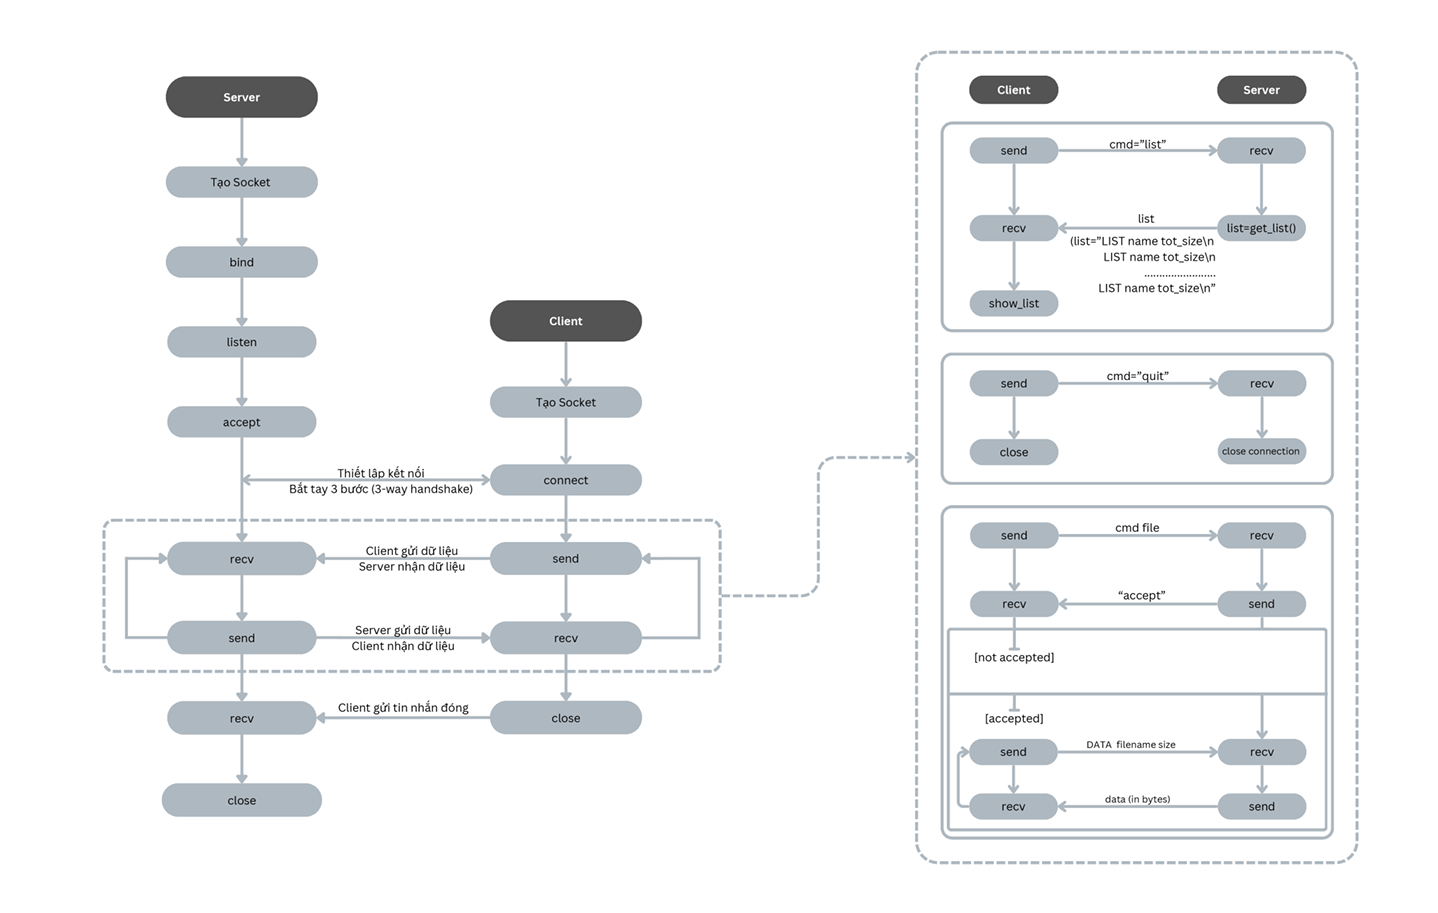
\includegraphics[width=0.8\textwidth]{Screenshorts/diagram.png}
          \caption{Sơ đồ minh họa kịch bản giao tiếp}\label{fig:diagram}
        \end{figure}
\end{itemize}

\pagebreak
\section{Các tính năng chương trình}
    \subsection{Các tính năng cơ bản}
      \begin{enumerate}
        \item Server phục vụ đồng thời nhiều Client cùng lúc.
        \item Client nhận được danh sách tài nguyên từ Server. 
        \item Thêm file mới vào danh sách  tải và thêm vào độ ưu tiên tải nếu muốn (Phần 2).
        \item Duyệt file mỗi khi tải xong từng file (Phần 1) và duyệt file mỗi 2 giây (Phần 2).
        \item Mỗi Client chỉ dùng duy nhất một kết nối để download tuần tự các phần nhỏ xen kẽ của từng file từ server (Phần 2).
        \item Hiển thị thanh tiến độ tải.
        \item Khi Client bấm "Ctrl + C" thì chương trình client đóng kết nối đến Server và kết thúc chương trình.
    \end{enumerate}
    \subsection{Các tính năng bổ sung}
    \begin{enumerate}
        \item Giao diện
        \item 
    \end{enumerate}

\pagebreak
\section{Hướng dẫn sử dụng tính năng chương trình}
\begin{description}
  \item \textbf{Chuẩn bị:} Cấu hình file \verb|.env| trước khi chạy chương trình (cấu hình cho Server và Client) và tải thư viện bổ sung bằng lệnh \verb|pip install -r requirements.txt| (trong thư mục \verb|Source|).
        \begin{itemize}
          \item \textbf{Server:}
                \begin{itemize}
                  \item \verb|HOST|: Địa chỉ IP của Server
                  \item \verb|PORT|: Cổng kết nối của Server
                  \item \verb|SERVER_RESOURCES_PATH|: Đường dẫn chứa tài nguyên có thể tải về
                \end{itemize}
          \item \textbf{Client:}
                \begin{itemize}
                  \item \verb|HOST|: Địa chỉ IP của Server
                  \item \verb|PORT|: Cổng kết nối của Server
                  \item \verb|CLIENT_DOWNLOADS_PATH|: Đường dẫn chứa tài nguyên đã tải về
                  \item \verb|CLIENT_REQUEST_INPUT|: Đường dẫn file chứa danh sách file cần tải về
                \end{itemize}
        \end{itemize}
  \item \textbf{Bước 1:} Chạy file \verb|server.py| bằng lệnh \verb|py server.py|, lúc này một Socket Server sẽ chạy và chờ các kết nối từ Client.\\Chạy file \verb|client.py| bằng lệnh \verb|py client.py| khởi tạo một Socket Client và tự động kết nối đến Server.
  \item \textbf{Bước 2:} Sau khi Client kết nối thành công, Server sẽ hiển thị địa chỉ của Client đã kết nối và gửi đi danh sách tài nguyên có thể tải về cho Client.
  \item \textbf{Bước 3:} Nhập những file muốn tải vào \verb|input.txt| trong đường dẫn của ứng dụng Client (mặc định ở \verb|Source/app/client/input.txt|). Client sẽ tự động đọc (mỗi 2s) và tải file trong danh sách theo mức độ ưu tiên được quy ước từ trước.\\ \\
        Ngoài ra còn có thể nhập lệnh bằng \verb|console| với quy tắc giao tiếp:
        \begin{itemize}
          \item \verb|"help", "h"|: khi gõ câu lệnh này Server sẽ trả lời \texttt{Show all commands} và in ra tất cả câu lệnh của commands.
          \item \verb|"quit", "q"|:  khi gõ câu lệnh này Server sẽ trả lời \texttt{Quit the program} và sẽ ngắt kết nối với Client.
          \item \verb|"list", "l"|:  khi gõ câu lệnh này Server sẽ trả lời \texttt{Get lists of available files from Server} và in ra danh sách các file có thể tải xuống từ server.
          \item \verb|"get", "g"|:  khi gõ lệnh này người dùng có thể tải file từ server theo tên file người dùng nhập bằng \verb|console|.
        \end{itemize}
  \item \textbf{Bước 4:} Ngắt kết nối bằng cách \verb|Ctrl+C| (có thể thực hiện ở cả server và client) hoặc nhập lệnh \verb|"q"| (chỉ ở client).
\end{description}

\pagebreak
\section{Bảng phân công việc}
\begin{center}
  \renewcommand{\arraystretch}{1.5}
  \begin{tabular}{|c|p{\dimexpr0.6\linewidth-2\tabcolsep}|c|}
    \hline
    \textbf{STT} & \textbf{Công việc}                                                                                         & \textbf{Người thực hiện} \\\hline
    \multicolumn{3}{|c|}{\textbf{Part I}}                                                                                                                \\\hline
    1            & Client có thể nhận được danh sách các file từ Server và ctrl-c                                             & 0,5                      \\\hline
    2            & Client có thể nhận lần lượt từng file thành công từ Server. Server có thể gửi file thành công tới Client   & 2                        \\\hline
    3            & Hiển thị percent download file và phát hiện những file cần download tiếp theo 2s quét file input.txt 1 lần & 0,5                      \\\hline
    \multicolumn{3}{|c|}{\textbf{Phần II}}                                                                                                               \\\hline
    4            & Client có thể nhận được danh sách các file từ Server và ctrl-c                                             & 0,5                      \\\hline
    5            & 2s quét file input.txt 1 lần                                                                               & 0,5                      \\\hline
    6            & Hiển thị percent download files                                                                            & 1                        \\\hline
    7            & Client có thể nhận files thành công từ Server. Tập tin sau khi download phải đúng và đủ dung lượng         & 3                        \\\hline
    8            & Độ ưu tiên CRITICAL, HIGH, NORMAL                                                                          & 1,5                      \\\hline
    9            & Viết báo cáo                                                                                               & 1,5                      \\\hline
  \end{tabular}
\end{center}

\pagebreak
\section{Ảnh chụp màn hình}
\begin{figure}[ht]
  \centering
  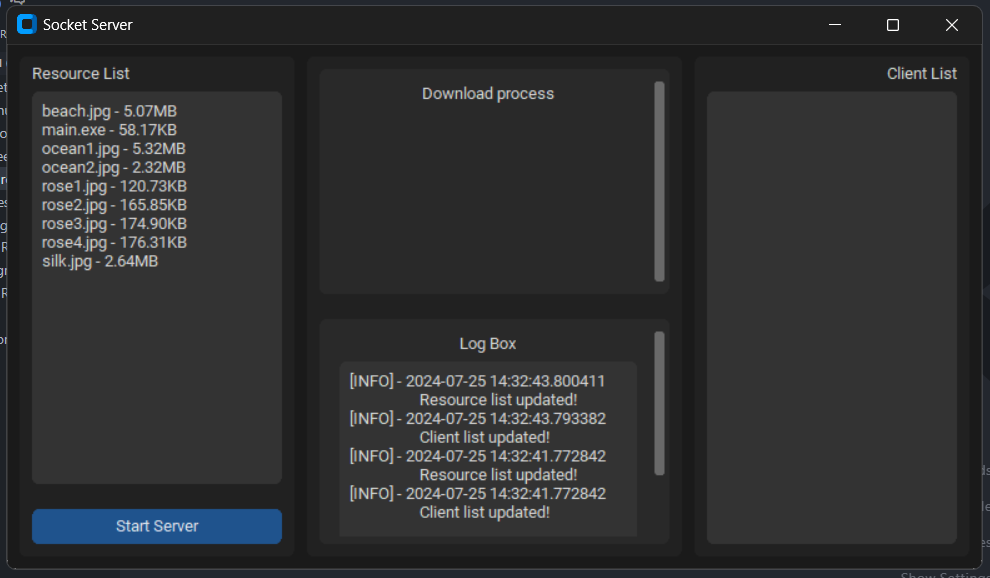
\includegraphics[width=0.8\textwidth]{Screenshorts/server-gui.png}
  \caption{Giao diện Server}\label{fig:server-gui}
\end{figure}

% References
\pagebreak
\section{Nguồn tham khảo}
\begin{enumerate}
    \item Mai Văn Cường - Trần Trung Dũng - Trần Hồng Ngọc - Lê Ngọc Sơn - Lê Giang 
Thanh - Trương Thị Mỹ Trang - Đào Anh Tuấn, Giáo trình Mạng máy tính, NXB 
Khoa học và Kỹ thuật, Xuất bản năm 2020
    \item Khoa Công nghệ thông tin – Trường ĐH Khoa học Tự nhiên, Slide Bài giảng môn 
Mạng máy tính, Tài liệu trực tuyến.
  \item \href{https://www.geeksforgeeks.org/}{geeksforgeeks}
  \item \href{https://stackoverflow.com/questions/47847392/keyboard-interrupt-sockets-and-threads}{Keyboard interrupt sockets and threads}
\end{enumerate}

\end{document}